\chapter{Validation}
\label{chap:validation}

\section{No ground truth}

To improve a segmentation, I had to be able to tell that it improved. Our 2018 masks are not a ground
truth: they encode our 2018 method, fat vessels included (Figure~\ref{fig:profile}). Expert annotation
is the usual answer, but none is available for this scan: I am no longer in touch with the researchers,
and annotating these images requires an expertise I do not have. Labels I painted myself would only
encode the algorithm's own assumptions.

I built two tools to address this. The first is ready for whoever can provide expert labels; the second
is the metric I actually used.

\paragraph{An annotation page} \code{tools/annotation} picks about ten crops of 256 pixels from a
segmentation (burst-rich, vessel-rich and random tissue), each with three slices of context on either
side, and serves a local web page (standard-library server, no extra dependency) to paint them
(Figure~\ref{fig:annotation}): brush, bucket fill, a ``wand'' that fills the connected pixels of
similar brightness (a click inside a vessel stops at its edge), undo, and an \emph{unsure} label excluded
from the scores. The view can be zoomed, panned and re-contrasted, the labels shown as outlines only,
the brush restricted to pixels of one label (to paint a vessel against bone without touching the bone),
and each crop carries a free-text note for doubts. Work is saved automatically. Crops can start from the current segmentation (much faster, but biased toward the algorithm,
which the manifest records). A \code{score} command then reports per-class agreement and the
confusion matrix against any segmentation.

\begin{figure}[ht]
  \centering
  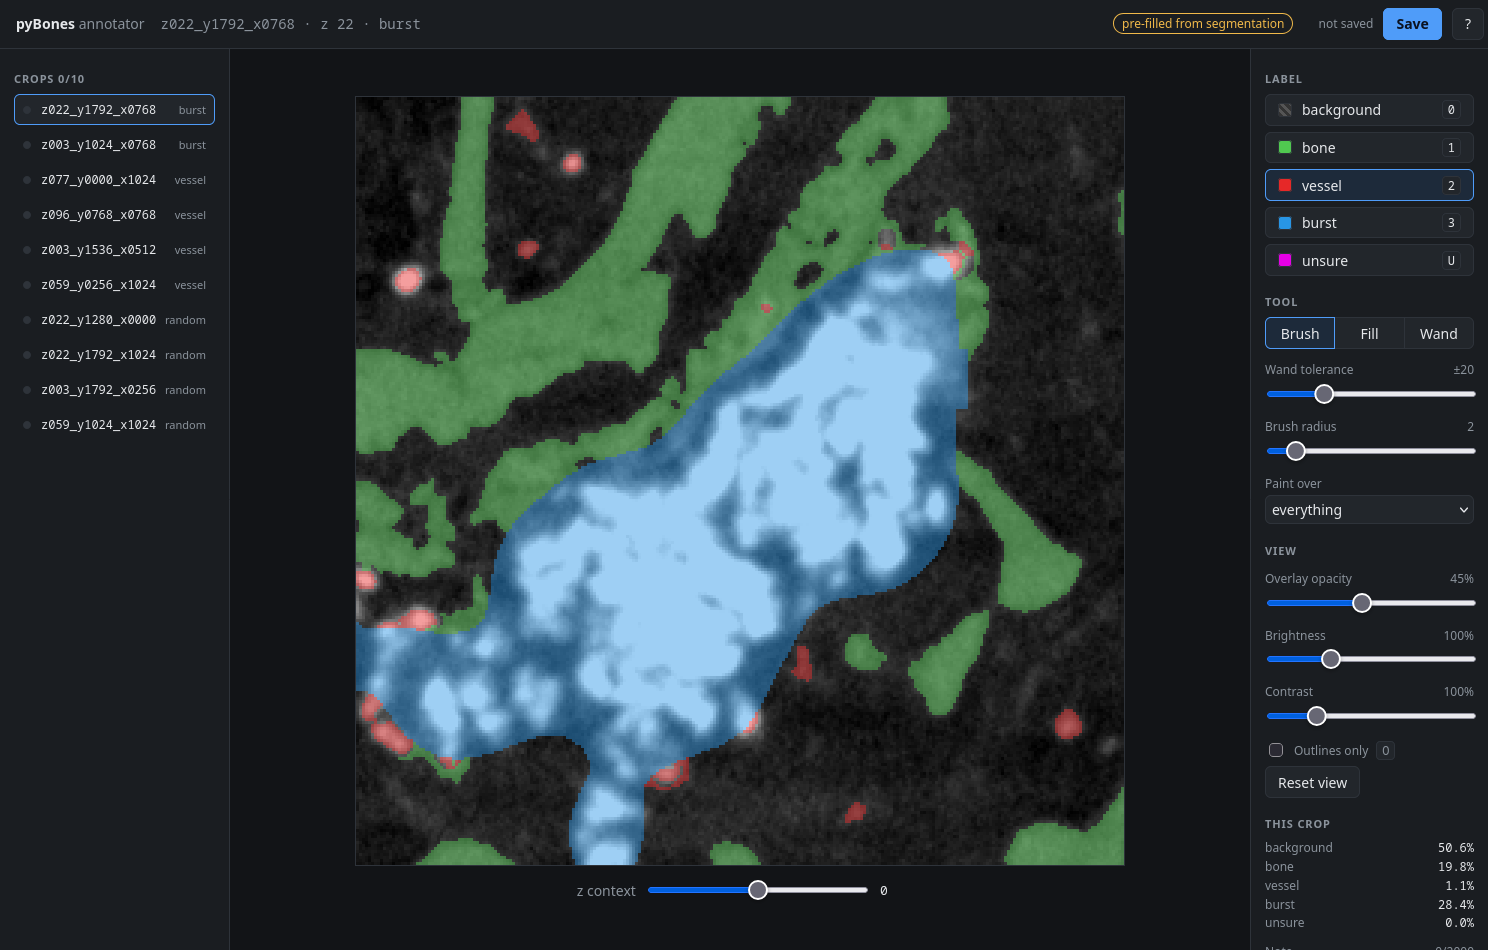
\includegraphics[width=0.85\linewidth]{../../screenshots/05-annotation-tool.png}
  \caption{The annotation page: crops on the left, the label palette and tools on the right; the
    arrow keys browse the neighbouring slices, the way a vessel is told from a trabecula by eye.}
  \label{fig:annotation}
\end{figure}

\section{A synthetic phantom}

\code{tools/phantom} renders a $\mu$CT-like volume ($96 \times 512 \times 512$ voxels of 3\um) whose
labels are known exactly:
\begin{itemize}
  \item cortex walls and trabecular plates (discs), and trabecular rods \emph{bridging} two plates;
  \item vessels as smooth random walks of tube segments of 3 to 25\um{} radius, some segments clotted
        (20 to 50\,\% filled), some empty (invisible, excluded from the scores);
  \item burst clusters: spheres of 110 to 200\um{} radius filled with dense speckles and a diffuse haze;
  \item every shape rendered with a partial-volume edge, then blurred and corrupted by noise.
\end{itemize}
Its parameters are calibrated on the real scan: the class intensities (medians of each class), the noise
(and its growth with intensity), the burst sizes, and the blur, measured on the real bone edges
($\sigma = 4.4$\um). A score reports, per class, the Dice coefficient (overlap), the precision (how much
of what was labelled is right) and the recall (how much of the truth was found), plus the vessel recall
per radius band and on clotted segments.

A phantom only helps if it is realistic, and mine was wrong twice during development. First, its rods
floated freely: the rule ``bone cannot float'' then labelled them as vessels, which no real rod does.
Second, its bursts were half the size of the real ones, below the detector's minimum area: the phantom
was unfair to the algorithm. I fixed both by measuring the real data (rod geometry, burst sizes)
before trusting a score again.

\begin{figure}[ht]
\centering
\panel{0.32}{phantom_raw.jpg}{Phantom slice.}\hfill
\panel{0.32}{phantom_truth.jpg}{Exact ground truth.}\hfill
\panel{0.32}{phantom_segmentation.jpg}{Segmentation (\pbValueVersion).}
\caption{A slice of the phantom. Today's scores: bone Dice \pbValueBoneDice, vessel Dice
  \pbValueVesselDice{} (precision \pbValueVesselPrecision, recall \pbValueVesselRecall), burst Dice
  \pbValueBurstDice; \pbValueAccuracy{} of all voxels correct.}
\label{fig:phantom}
\end{figure}

\section{Every version, on the same ground truth}

I recorded each milestone of the rewrite as a commit of my development repository.
\code{python -m tools.report history} checks each of them out in its own git worktree, with its own
environment, runs it on the \emph{current} phantom and scores it with today's scorer. The comparison
is therefore fair: same input, same metric, only the code changes (Table~\ref{tab:history},
Figure~\ref{fig:history}). The published repository starts from the final state and does not hold
those commits: their scores and the few slices the figures show are kept as an archive
(\code{docs/report/data/}), and only the current version is run again.

\begin{table}[ht]
\centering
\small
\begin{tabular}{@{}l l r r r r r r@{}}
\toprule
Version & Commit & Bone & Vessel & (prec.) & (recall) & Burst & Real stack \\
\midrule
First Python port (2D, per-slice) & \texttt{6e040e7} & 0.972 & \textbf{0.709} & 0.569 & 0.943 & 0.887 & 4\,s / 0.3\,GB \\
3D connectivity refinement & \texttt{3d05cea} & 0.975 & \textbf{0.674} & 0.521 & 0.953 & 0.884 & 12\,s / 0.8\,GB \\
3D burst density & \texttt{222b1a4} & 0.975 & \textbf{0.686} & 0.536 & 0.953 & 0.897 & 12\,s / 1.2\,GB \\
Physical units, analytic kernels & \texttt{fe645dd} & 0.974 & \textbf{0.685} & 0.535 & 0.954 & 0.897 & -- \\
Half-maximum vessel edges & \texttt{50a394c} & 0.986 & \textbf{0.810} & 0.719 & 0.928 & 0.897 & 12\,s / 1.3\,GB \\
Tube-vs-plate veto & \texttt{427cd3d} & 0.989 & \textbf{0.829} & 0.753 & 0.923 & 0.897 & 33\,s / 3.0\,GB \\
3D vessel halo & \texttt{e7ca4a1} & 0.989 & \textbf{0.837} & 0.776 & 0.907 & 0.897 & -- \\
Half-maximum burst boundary & \texttt{d33da52} & 0.989 & \textbf{0.840} & 0.801 & 0.884 & 0.911 & -- \\
Current code (0.7.0) & -- & 0.989 & \textbf{0.862} & 0.826 & 0.901 & 0.922 & 24\,s / 1.7\,GB \\
\bottomrule
\end{tabular}

\caption{Dice score per class on the phantom for every milestone of the rewrite, vessel precision and
  recall, and the cost of segmenting the real stack (wall time and peak memory, all measured on the
  machine described in Chapter~\ref{chap:performance}; ``--'' when that version was not run on the real
  data).}
\label{tab:history}
\end{table}

\begin{figure}[ht]
\centering
\begin{tikzpicture}
\begin{axis}[width=0.95\linewidth,height=6cm,ymin=0.6,ymax=1.0,ylabel={Dice},
  xtick=data,xticklabels from table={\historytable}{key},
  xticklabel style={rotate=35,anchor=east,font=\footnotesize\ttfamily},
  legend style={font=\footnotesize,at={(0.5,-0.38)},anchor=north,legend columns=3,draw=none},
  tick label style={font=\small},label style={font=\small},grid=major,grid style={muted!20}]
  \addplot[boneC!70!black,thick,mark=*] table[x expr=\coordindex,y=bone_dice]{\historytable};
  \addlegendentry{bone}
  \addplot[vesselC,thick,mark=*] table[x expr=\coordindex,y=vessel_dice]{\historytable};
  \addlegendentry{vessel}
  \addplot[burstC,thick,mark=*] table[x expr=\coordindex,y=burst_dice]{\historytable};
  \addlegendentry{burst}
\end{axis}
\end{tikzpicture}
\caption{Dice per class along the history of the rewrite (same phantom, same scorer).}
\label{fig:history}
\end{figure}

I read the history as follows.
\begin{itemize}
  \item The \textbf{first port} (0.1, close in spirit to 2018 but with global thresholds and labelled
        bursts) already finds most vessels (high recall) but labels far too much as vessel (precision
        about 0.57): the vessels are fat.
  \item The \textbf{3D refinement} of 0.2 \emph{lowered} the vessel score at first, which surprised me. It turned many
        ambiguous blobs into vessels, which was right in spirit but only added more voxels to vessels
        that were already too thick. A better decision rule cannot fix wrong edges.
  \item The \textbf{half-maximum edges} are the turning point: the largest single gain of the rewrite,
        on vessels and on bone alike. Physics beat parameter tuning.
  \item The \textbf{plate veto}, the \textbf{3D halo} and the \textbf{burst boundary} each add a
        smaller, measured gain. Today's version measures that boundary in 3D: bursts no longer follow
        and hollow out the vessels lying in a slice (Section~\ref{sec:bursts}), which raises both the
        vessel and the burst scores; earlier, it had become faster and lighter (tubularity computed
        only where it is used).
\end{itemize}

\begin{figure}[ht]
\centering
\begin{tikzpicture}
\begin{axis}[width=0.95\linewidth,height=5.5cm,ymin=0,ymax=1.0,ylabel={vessel recall},
  xtick=data,xticklabels from table={\historytable}{key},
  xticklabel style={rotate=35,anchor=east,font=\footnotesize\ttfamily},
  legend style={font=\footnotesize,at={(0.5,-0.38)},anchor=north,legend columns=4,draw=none},
  tick label style={font=\small},label style={font=\small},grid=major,grid style={muted!20}]
  \addplot[vesselC!40,thick,mark=*] table[x expr=\coordindex,y=vessel_recall_0_6um]{\historytable};
  \addlegendentry{radius 0--6\um}
  \addplot[vesselC!70,thick,mark=*] table[x expr=\coordindex,y=vessel_recall_6_12um]{\historytable};
  \addlegendentry{radius 6--12\um}
  \addplot[vesselC,thick,mark=*] table[x expr=\coordindex,y=vessel_recall_12_25um]{\historytable};
  \addlegendentry{radius 12--25\um}
  \addplot[ink,thick,dashed,mark=o] table[x expr=\coordindex,y=clotted_recall]{\historytable};
  \addlegendentry{clotted segments}
\end{axis}
\end{tikzpicture}
\caption{Vessel recall per radius band and on clotted segments. Thin vessels are found far less often
  than large ones (Section~\ref{sec:thin}); the recall of large vessels decreases slightly as their
  edges become exact (fat masks ``find'' every truth voxel).}
\label{fig:history-recall}
\end{figure}

\section{On the real scan}

Figure~\ref{fig:real-overview} compares the 2018 masks with today's segmentation on a whole slice, and
Figure~\ref{fig:real-evolution} follows one region through the versions. Today, the stack is
\pbValueFracBone\,\% bone, \pbValueFracVessel\,\% vessel and \pbValueFracBurst\,\% burst.

\begin{figure}[ht]
\centering
\panel{0.4}{overview_legacy.jpg}{2018 masks (bone, vessels; bursts were discarded).}\hspace{0.05\linewidth}
\panel{0.4}{overview_current.jpg}{Version \pbValueVersion{} (bone, vessels, bursts).}
\caption{Slice 0, the 2018 segmentation and today's.}
\label{fig:real-overview}
\end{figure}

\begin{figure}[p]
\centering
\panel{0.32}{evolution_marrow_raw.jpg}{Raw.}\hfill
\panel{0.32}{evolution_marrow_legacy.jpg}{2018 (Matlab).}\hfill
\panel{0.32}{evolution_marrow_v01.jpg}{0.1: first port.}\\[6pt]
\panel{0.32}{evolution_marrow_v02.jpg}{0.2: 3D refinement.}\hfill
\panel{0.32}{evolution_marrow_halfmax.jpg}{Half-maximum edges.}\hfill
\panel{0.32}{evolution_marrow_current.jpg}{\pbValueVersion.}
\caption{One marrow region through the versions. 2018: fat vessels, bursts left unlabelled. 0.1: bursts
  found, but thin dim vessels lost to bone. 0.2: vessels back, still fat and wrapped in bone. Half-maximum
  edges and the later steps: vessels at their visible width, trabeculae untouched.}
\label{fig:real-evolution}
\end{figure}
